\section{Generierung von Vorschlägen für Testdaten}\label{chap:testdatasuggestions}

Es gibt verschiedene Strategien dem Entwickler repräsentative Testwerte vorzuschlagen, die die Variationspunkte eines SQL-Statements beeinflussen.
Als Grundlage dafür dient neben dem Quellcode auch das Datenbanksystem mit den enthaltenen Echtdaten.
In den folgenden Beispielen werden Unternehmensdaten aus einer SAP-Infrastruktur genutzt.
Die Integration solcher Datenbanksysteme und die Administration der genutzten Testdaten werden in Kapitel \ref{chap:testdataadministration} ausführlicher behandelt.

Neben der Betrachtung der Charakteristiken von Daten innerhalb der Datenbank und dem Kontext aus dem Quellcode ist vor allem die Verknüpfung mit Analyseergebnissen, vorrangig den Laufzeitmessungen, ein Kriterium für die Generierung der Vorschläge.
Mittels Auswahl unterschiedlicher, vorgeschlagener Testwerte ist es dem Entwickler möglich, konkrete Ausprägungen von SQL-Statements nachzuvollziehen und auf Grundlage der Auswertung der Messungen gegebenenfalls Optimierungen durchzuführen bis das gewünschte Performance-Verhalten erreicht ist.
Doch zuerst müssen die Variablen ermittelt werden, die einen Einfluss auf das SQL-Statement haben.

\subsection{Bestimmung der zu betrachtenden Variablen}
Kapitel \ref{sec:controlflowandsqldependencies} zeigte bereits auf, dass Variablen auf unterschiedliche Weisen auf ein SQL-Statement einwirken können.
Dies schlägt sich auch auf die Vorschlagsgenerierung nieder.
Um die Variablen, die auf ein SQL-Statement Einfluss nehmen, zu bestimmen, dient die Schnittstelle \texttt{javascriptParser.getSqlQueryAtPosition()} des Quellcode-Parsers \cite{Horschig2014}.
Sie liefert ein Objekt mit zwei wichtigen Attributen zurück: \texttt{dependencies} und \texttt{variables}.
Dabei enthält \texttt{dependencies} alle Variablen, von denen das SQL-Statement im Kontrollfluss abhängig ist, wohingegen \texttt{variables} alle Variablen umfasst, die innerhalb des SQL-Statements auftreten.
Darüber hinaus können Variablen auch in beiden Listen vorkommen (die Verknüpfung erfolgt in diesem Fall anhand des Attributs \texttt{uniqueName}).
Die Elemente in \texttt{variables} enthalten zusätzlich Kontextinformationen, die eine Zuordnung zu Spalten innerhalb einer Relation ermöglichen, und so die Grundlage für die Generierung von Testdatenvorschlägen schaffen.
In Abbildung \ref{fig:querytree} ist eine solche Datenstruktur beispielhaft für Code-Beispiel \ref{lst:differentdep} dargestellt.

\begin{figure}[ht]
	\centering
	\scalebox{.58}{
		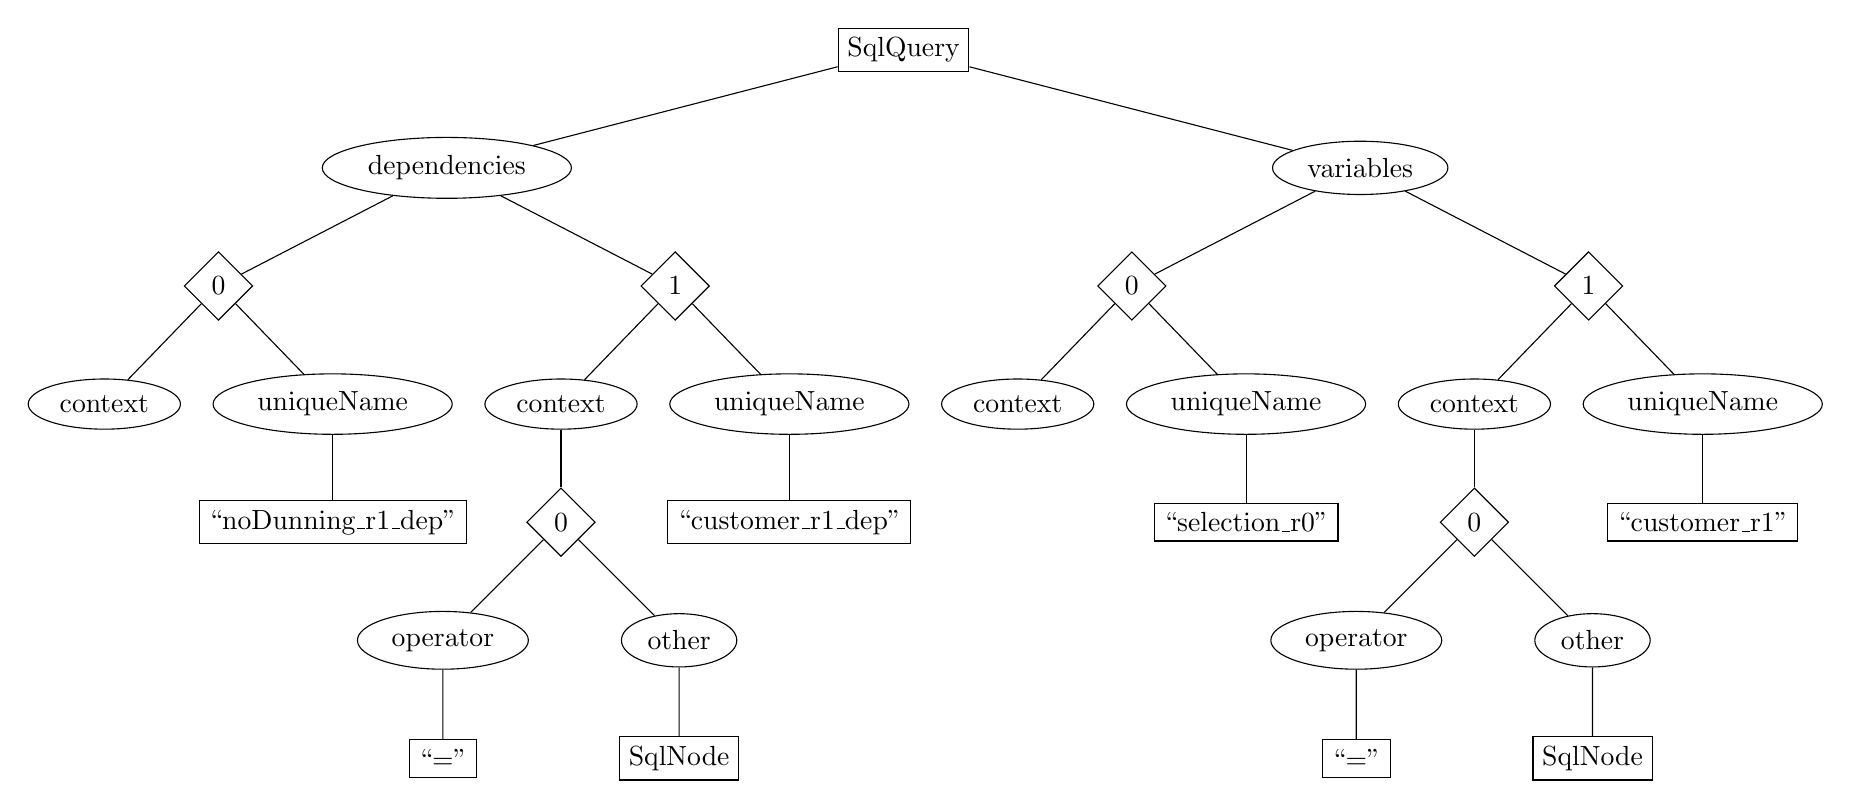
\begin{tikzpicture}
			\usetikzlibrary{shapes}
			\tikzstyle{e} = [draw, shape=ellipse]
			\tikzstyle{r} = [draw, shape=rectangle]
			\tikzstyle{d} = [draw, shape=diamond]
			\node[r] (is-root) {SqlQuery}
				[sibling distance=11.6cm]
				child {
					node[e] {dependencies}
					[sibling distance=5.8cm]
					child {
						node[d] {0}
						[sibling distance=2.9cm]
						child { node[e] {context} }
						child {
							node[e] {uniqueName}
							child { node[r] {``noDunning\_r1\_dep''} }
						}
					}
					child {
						node[d] {1}
						[sibling distance=2.9cm]
						child {
							node[e] {context}
							child {
								node[d] {0}
								[sibling distance=3cm]
								child {
									node[e] {operator}
									child { node[r] {``=''} }
								}
								child {
									node[e] {other}
									child { node[r] {SqlNode} }
								}
							}
						}
						child {
							node[e] {uniqueName}
							child { node[r] {``customer\_r1\_dep''} }
						}
					}
				}
				child {
					node[e] {variables}
					[sibling distance=5.8cm]
					child {
						node[d] {0}
						[sibling distance=2.9cm]
						child {
							node[e] {context}
						}
						child {
							node[e] {uniqueName}
							child { node[r] {``selection\_r0''} }
						}
					}
					child {
						node[d] {1}
						[sibling distance=2.9cm]
						child {
							node[e] {context}
							child {
								node[d] {0}
								[sibling distance=3cm]
								child {
									node[e] {operator}
									child { node[r] {``=''} }
								}
								child {
									node[e] {other}
									child { node[r] {SqlNode} }
								}
							}
						}
						child {
							node[e] {uniqueName}
							child { node[r] {``customer\_r1''} }
						}
					}
				};
		\end{tikzpicture}
	}

	\vspace{\baselineskip}

	\scalebox{1}{
		\begin{tikzpicture}[framed, node distance=2cm]
			\usetikzlibrary{shapes}
			\tikzstyle{e} = [draw, shape=ellipse]
			\tikzstyle{r} = [draw, shape=rectangle]
			\tikzstyle{d} = [draw, shape=diamond]
			%\node [e] {dependencies};

			\node (title) [font=\bfseries] {Legende:};
			\node [r, right = of title, label=right:{Objekt}] (object) {};
			\node [e, right = of object, label=right:{Attribut}] (attribute) {};
			\node [d, right = of attribute, label=right:{Array-Element}] (array) {};
		\end{tikzpicture}
	}

	\caption{Datenstruktur zum Code-Beispiel \ref{lst:differentdep}}
	\label{fig:querytree}
\end{figure}


\subsection{Vorschläge auf Basis von Datencharakteristiken}\label{chap:datacharacteristics}
Sobald Variablen nicht nur die Gestalt eines SQL-Statements variieren, sondern auch darin einfließen, ist der erste Anhaltspunkt für das Vorschlagen relevanter Testwerte die Charakteristik der Datenbankinhalte.
Für Selektionsfilter spielen dabei primär die Verteilung der Daten innerhalb der Relationen sowie die Anzahl ihrer unterschiedlichen Werteausprägungen eine Rolle.
Im Gegensatz dazu werden für die Projektion, Sortierung und Gruppierung Metainformationen zu den Relationen der Datenbank berücksichtigt.
Zweiteres wird in Kapitel \ref{chap:databasemeta} näher betrachtet.

%\begin{figure}
%\centering
	%\begin{tikzpicture}
		%\begin{axis}[
				%axis lines=left,
				%width  = 0.85*\textwidth,
				%height  = 6cm,
				%symbolic x coords={Males,Females},
				%xtick=data,
				%enlarge x limits=0.5,
				%bar width=40pt,
				%ybar,
				%ylabel={Percentage},
				%ymin=0.0,
				%ymax=100.0,
				%]
				%\addplot[ybar,fill=light-gray] coordinates {
						%(Males,55)
						%(Females,45)
				%};
		%\end{axis}
	%\end{tikzpicture}
	%\caption{(TODO: ersetzten durch statistik in BSEG.) Verteilung der Werte in der Spalte Gender.}
	%\label{fig:gender}
%\end{figure}

\pgfkeys{
    /pgf/number format/precision=0,
    /pgf/number format/fixed zerofill=true,
    /pgf/number format/fixed,
		/pgf/number format/.cd,
		use comma,
		1000 sep={.}
}

\begin{figure}[ht]
\centering
	\begin{tikzpicture}
		\begin{axis}[
			axis lines=left,
			xbar, xmin=0,
			width=0.85*\textwidth,
			height=6cm,
			enlarge y limits=0.1,
			xlabel={Absolute Anzahl distinkter Werte},
			symbolic y coords={MANDT,GJAHR,ZLSCH,BUKRS,AUGDT,LIFNR,SKFBT,KUNNR,WRBTR,BELNR},
			ytick=data,
			bar width=5pt,
			nodes near coords, nodes near coords align={horizontal},
			]
			\addplot[fill=light-gray] coordinates {
				(5636590,BELNR)
				(560628,WRBTR)
				(408015,KUNNR)
				(228722,SKFBT)
				(48407,LIFNR)
				(2304,AUGDT)
				(71,BUKRS)
				(31,ZLSCH)
				(10,GJAHR)
				(2,MANDT)
			};
		\end{axis}
	\end{tikzpicture}
	\caption{Verteilung distinkter Werten einer Auswahl von Spalten aus BSEG}
	\label{fig:bseg}
\end{figure}

Abbildung \ref{fig:bseg} zeigt eine Auswahl der 326 Spalten der BSEG-Relation mit der Anzahl deren distinkter Werte eines SAP-Systems.
Die Relation enthält alle einzelnen Belegpositionen zu den Buchungsbelegen des Unternehmens.
Eine Erläuterung zu den Bedeutungenn der einzelnen Spalten befindet sich im Anhang (Tabelle \ref{tab:bsegerlaeuterung}).

Besonders auffällig ist die starke Varianz der Anzahl von distinkten Werten im Vergleich der verschiedenen Spalten.
Sollte die Anzahl der distinkten Werte einstellig sein (beispielsweise bei der Spalte MANDT), können dem Entwickler alle möglichen Ausprägungen in einem Auswahlmenü zur Verfügung gestellt werden.
Damit wird gleichzeitig auch sichergestellt, dass nur Werte eingegeben werden können, die beim testweisen Ausführen des SQL-Statements ein Ergebnis zurückgeben.
Auf der anderen Seite können sich Spalten jedoch über eine große Menge von verschiedenen Datenausprägungen erstrecken, wie zum Beispiel bei Belegnummern (BELNR), was eine einfache Auswahl passender Testdaten kompliziert gestaltet.
Für diesen Fall werden Äquivalenzklassen anhand der Vorkommen der Werte erzeugt. Die Klassen von Bedeutung umfassen die drei häufigsten Werte, die drei seltensten Werte und drei Werte um den Median.

Für die häufigsten Werte wird eine aufsteigende Sortierung anhand der Anzahl ihres Vorkommens vorgenommen und die ersten drei selektiert.
Sollten mehrere Werte dieselbe Anzahl an Vorkommen vorweisen, werden sie zusätzlich anhand ihrer Werte aufsteigend sortiert.
Im Unterschied dazu wird bei der Klasse der seltensten Werten initial eine absteigende Sortierung vorgenommen.
Für die Werte um den Median muss zuerst die Anzahl der verschiedene Werte ermittelt werden.
Anschließend dient die Halbierung des sortierten Ergebnisses als Offset für die Bestimmung der drei vorzuschlagenden Werte.
Die SQL-Statements dazu befinden sich als Code-Beispiel \ref{lst:distinctvalues} im Anhang.

\subsection{Vorschläge anhand von Metainformationen}\label{chap:databasemeta}
Für Projektion, Sortierung oder Gruppierung sind weniger die Spalteninhalte wichtig, als vielmehr die Spalten an sich.
Um Vorschläge für diese Art SQL-Statement-Variablen zu erzeugen, werden anhand der Metainformationen über Spalten der betrachteten Relation aus der SAP HANA-internen Systemtabelle \texttt{SYS.TABLE\_COLUMNS} die Spaltennamen bestimmt (vgl. Code-Beispiel\ref{lst:hanasys}).
\begin{lstlisting}[caption={SQL-Statement für Metainformationen zu Relationen}, label={lst:hanasys}, language=mySQL]
	SELECT COLUMN_NAME
	FROM SYS.TABLE_COLUMNS
	WHERE SCHEMA_NAME = '<schema>'
	AND TABLE_NAME = '<table>'
\end{lstlisting}
Die notwendigen Informationen (Schema und Relation) werden dazu dem SQL-Statement entnommen.

\subsubsection{Nutzung von Metainformationen für UI-Elemente}
Die Metainformationen zu Spalten umfassen neben den Namen auch weitere nützliche Informationen, die die Eingabe von Testdaten unterstützen können.
Beispielsweise können der Datentyp von Spalten (\texttt{DATA\_TYPE\_NAME}), die Erlaubnis der Eingabe von NULL-Werten (\texttt{IS\_NULLABLE}) oder auch die maximale Länge für Eingaben in der betreffenden Spalte (\texttt{LENGTH}) für die Erstellung der Eingabefelder genutzt werden kann.
So kann die Eingabe, die eine Spalte mit Datumsangaben referenziert, durch einen Kalender vereinfacht werden.
Auch die Einschränkung auf Datentypen, z.B. Ganzzahlen, kann fehlerhafte Eingabe durch den Entwickler verhindern.
Eine weitere Unterstützung ist die Autovervollständigung von teilweise eingegebenen Werten.
Mittels des SQL-Operators \texttt{LIKE} kann dazu nach Daten gesucht werden, die dem Muster der bisherigen Eingabe entsprechen.
Diese Zusatzinformationen erhöhen zusammenfassend also den Komfort der Eingabe und können fehlerhafte Eingaben reduzieren.

\subsection{Adaptive Vorschlagsgenerierung durch Laufzeitanalysen}\label{chap:adaptive}
Der in Kapitel \ref{chap:datacharacteristics} vorgestelle Ansatz zum Vorschlagen einzelner Testwerte stößt an seine Grenzen, sobald mehrere Parameter genutzt werden und diese voneinander abhängig sind.
Im Code-Beispiel \ref{lst:dynamicsql} aus Kapitel \ref{sec:dependencydetection} werden beispielsweise offene Belege und deren Einzelpositionen gesucht.
Die Variable \texttt{customer} gibt dabei die Kundennummer an, mit der die Rechnungen assoziiert sind.
Wird zusätzlich ein Wert für \texttt{customerTo} festgelegt, erfolgt die Selektion anhand einer Bereichsanfrage.
Man kann nun annehmen, dass die Kundennummern mit den größten Gesamtsummen auch die meisten Belege bzw. Belegposition haben.
Tabelle \ref{tab:vergleichkonstellationen} verdeutlicht das Gegenteil.

\begin{table}[ht!]
	\centering
	\begin{tabular}{ |c|c|c|r| }
		\hline
		%\multicolumn{2}{|c|}{BSEG-Spalten} \\
		Kundennummer & Belege & Belegpositionen & Summe der Beträge\\
		\hline
		0000001201 & 12.555 & 19.449 & 72.160.054,92 \\
		0000003401 & 11.896 & 19.329 & 54.318.123,25 \\
		0000003501 & 12.380 & 24.571 & 52.813.094,78 \\
		\hline
		0016207834 & 246 & 273 & 5.930.616.840,00 \\
		0015423702 & 29 & 31 & 5.306.744.980,00 \\
		0000001051 & 4.750 & 7.617 & 5.159.057.217,21 \\
		\hline
	\end{tabular}
	\caption{Auswahl an Einträgen der BSEG-Relation nach Kundennummer}
	\label{tab:vergleichkonstellationen}
\end{table}

Im oberen Teil der Tabelle sind die drei Kundennummern gelistet, die die meisten Belegpositionen umfassen.
Der untere Teil enthält die Kundennummern mit den höchsten Gesamtsummen.
Es gibt zwei Auffälligkeiten: die Belege haben im Durchschnitt nur sehr wenige Positionen und viele Belege bzw. Belegpositionen haben nicht automatisch eine hohe Gesamtsumme zur Folge.
Würden nun Entscheidungen auf dieser Grundlage gefällt werden, z.B. zusätzliche Berechnungen für Kunden mit einem Umsatzvolumen von über 1 Milliarde \euro{}, würden einfache Testwertvorschläge diesen Teilbereich nicht abdecken.

Diese noch recht einfache Abhängigkeit kann beliebig erweitert werden.
Damit entstehen komplexe SQL- und Programmstrukturen, die durch das einfache Vorschlagen anhand von Charakteristiken einzelner Spalten nicht zwangsläufig die Randfälle aufzeigen, die der Entwickler sucht.
Aus diesem Grund ist die Betrachtung von Messergebnissen aus Laufzeitanalysen (\cite{Exner2014}, \cite{Mues2014}) eine sinnvolle Erweiterung, um die Genauigkeit bzw. den Nutzen der Vorschläge zu steigern.
Die variablen Stellen von SQL-Statements werden dabei durch die vom Entwickler ausgewählten Werte gefüllt.
Im nächsten Schritt werden nun diese atomaren Vorschläge kombiniert und mit dem dazugehörigen Ergebnis aus der Laufzeitanalyse verknüpft.
Dies ermöglicht die Vergleichbarkeit verschiedener Konstellationen.
Für die Erstellung der initialen Daten können zwei verschiedene Ansätze verfolgt werden.

Der offensichtliche Ansatz ist das Durchprobieren und Messen aller Kombinationen (Brute-Force).
Der hohe Aufwand, besonders bei Relationen mit vielen Einträgen und distinkten Werten in den Spalten, stellt jedoch aufgrund der enormen Berechnungszeit ein großes Hindernis dar.
Beispielsweise entstehen schon bei der Betrachtung von 3 Spalten mit jeweils 1000 distinkten Werten (typisch für z.B. Identifikationsmerkmale) eine Milliarde Kombinationen, die analysiert werden müssen.

Dem gegenüber steht der adaptive Ansatz, bei dem der Testdatenbestand kontinuierlich erweitert wird.
Diese Variante speichert die Ergebnisse der Laufzeitanalysen mit den dazugehören Testdatenkonstellationen als Testdatensets.
Sobald mehrere dieser Sets vorhanden sind, können dem Entwickler drei Vorauswahloptionen gegeben werden: das Testdatenset mit der höchsten Laufzeit, mit der geringsten Laufzeit und mit mittlerer Laufzeit.

Um für diese Methode eine Datengrundlage zu schaffen, stehen wiederum zwei Verfahren zur Auswahl.
Mithilfe der in Kapitel \ref{chap:datacharacteristics} ermittelten Werte können alle möglichen Kombinationen von Tupelausbildungen erstellt werden.
Dies entspricht einer Permutation der Werte aller betrachteten Spalten.
Allerdings entsteht somit dasselbe Problem wie bei der Brute-Force-Methode: mit steigender Anzahl an Spalten wächst die Anzahl der zu betrachtenden Tupel, selbst wenn diese keine Repräsentationen in der Relation vorweisen.

Aus diesem Grund werden die distinkten Kombinationen der betrachteten Spalten mit dem meisten Vorkommen innerhalb der Relation bestimmt (siehe Code-Beispiel \ref{lst:disinctcombinations}).
In Hinblick auf die Laufzeit der Analysen der einzelnen Kombinationen, wurde eine derzeitige Obergrenze von 50 zu betrachtenden Tupeln festgelegt.
Sollten Spalten über mehrere Relationen hinweg betrachtet werden, so erfolgt die Bestimmung auf Basis der Verknüpfung der Relationen.

\begin{lstlisting}[caption={Bestimmung distinkter Tupel anhand gegebener Spalten}, label={lst:disinctcombinations}, language=mySQL]
	SELECT TOP 50 DISTINCT <list of columns>, COUNT(*) AS OCCURENCES
	FROM <table>
	GROUP BY <list of columns>
	ORDER BY OCCURENCES DESC
\end{lstlisting}

%Anschließend werden die gefundenen Tupel zur Analyse ihrer Laufzeit der Datenbankabfrage genutzt.
Die gefundenen Tupel bilden mit Ergebnissen der Laufzeitanalysen die initialen Testdatensets, die durch die explorative Eingabe weiterer Werte durch den Entwickler kontinuierlich in ihrer Genauigkeit verbessert werden können.
Sollten neue Konstellationen von Testwerten vorliegen, werden diese als Sets mitsamt ihrer Laufzeit in der Datenbank der Web-IDE hinterlegt.
Die Ermittlung der Vorschläge an Testdatensets mit höchster, mittlerer und langsamster Laufzeit erfolgt durch Sortierung und Filterung anhand der gespeicherten Laufzeit.

%
%Durch explorative Eingabe weiterer Werte durch den Entwickler kann anschließend das Datenmodell kontinuierlich erweitert und zunehmend verbessert werden, zu sehen im Code-Beispiel \ref{lst:developerinput}.
%
%\begin{lstlisting}[caption={Eingaben von Testwertkonstellationen erweitern gegebenenfalls das Datenmodell}, label={lst:developerinput}, language=Python]
	%hier
	%kommt
	%der
	%algorithmus
	%rein
%\end{lstlisting}
%
%TODO: Algorithmus beschreiben.

%\subsection{Betrachtung von Zeitbereichsanfragen}
%Ein typischer Bestandteil von Datenbankanfragen in Geschäftsanwendungen sind Bereichsfilter mittels \texttt{column BETWEEN x AND y},  insbesondere für Zeiträume.
%Der in Kapitel \ref{chap:datacharacteristics} vorgestellte Algorithmus generiert Vorschläge basierend auf binären Operationen (zumeist Vergleiche), wohingegen ein Bereichsfilter ternär ist: er hat eine Wertuntergrenze, eine Wertobergrenze und eine Referenz auf eine Spalte.
%Deshalb ist eine besondere Betrachtung für passende Vorschläge sinnvoll.
%
%Sollte eine Bereichsanfrage erkannt werden, die eine Spalte vom Datentyp \texttt{DATE} referenziert, so kann der Entwickler eine vorgeschlagene Zeitraumgröße (z.B. eine Woche, ein Monat oder ein Jahr) auswählen oder selbst festlegen.
%Anschließend wird die referenzierte Spalte mithilfe der angegebenen Zeitraumgröße gescannt, ähnlich dem Prinzip des Sliding Window\footnote{\url{http://en.wikipedia.org/wiki/Sliding_window_protocol}}.
%Auf dieser Basis werden, ähnlich dem Algorithmus aus Kapitel \ref{chap:datacharacteristics}, bis zu 3 Vorschläge für die größte, kleinste und mittlere Anzahl an Resultaten erzeugt.
%Alternativ steht es dem Entwickler offen, Start- und Enddatum eigenständig festzulegen.

\nomenclature{AST}{Abstract Syntax Tree}
\subsection{Vorschläge für Variablenwerte ohne Datenbankbezug}
Nicht immer müssen Variablen in ein SQL-Statement einfließen, um darauf Auswirkungen zu haben.
Ein typisches Beispiel ist die Verwendung einer Variable als Bedingung, z.B. für Verzweigungen, zu sehen im Code-Beispiel \ref{lst:differentdep} in der Nutzung der Variable \texttt{noDunning}.
Das Setzen der Variable entscheidet über die Ergänzung des Selektionsfilters um die Bedingung \texttt{BSEG.MANST = 0}.
Sie hat jedoch keinen Bezug zu einem Attribut aus der Datenbank.
Für solche Fälle wird der Programmkontext der Variable für die Vorschläge der dazugehörigen Testwerte genutzt.
Abbildung \ref{fig:querytreeextended} zeigt für das Code-Beispiel \ref{lst:differentdep} die notwendige Erweiterung des Baumes aus Abbildung \ref{fig:querytree}.

\begin{figure}[ht!]
	\centering
	\scalebox{.58}{
		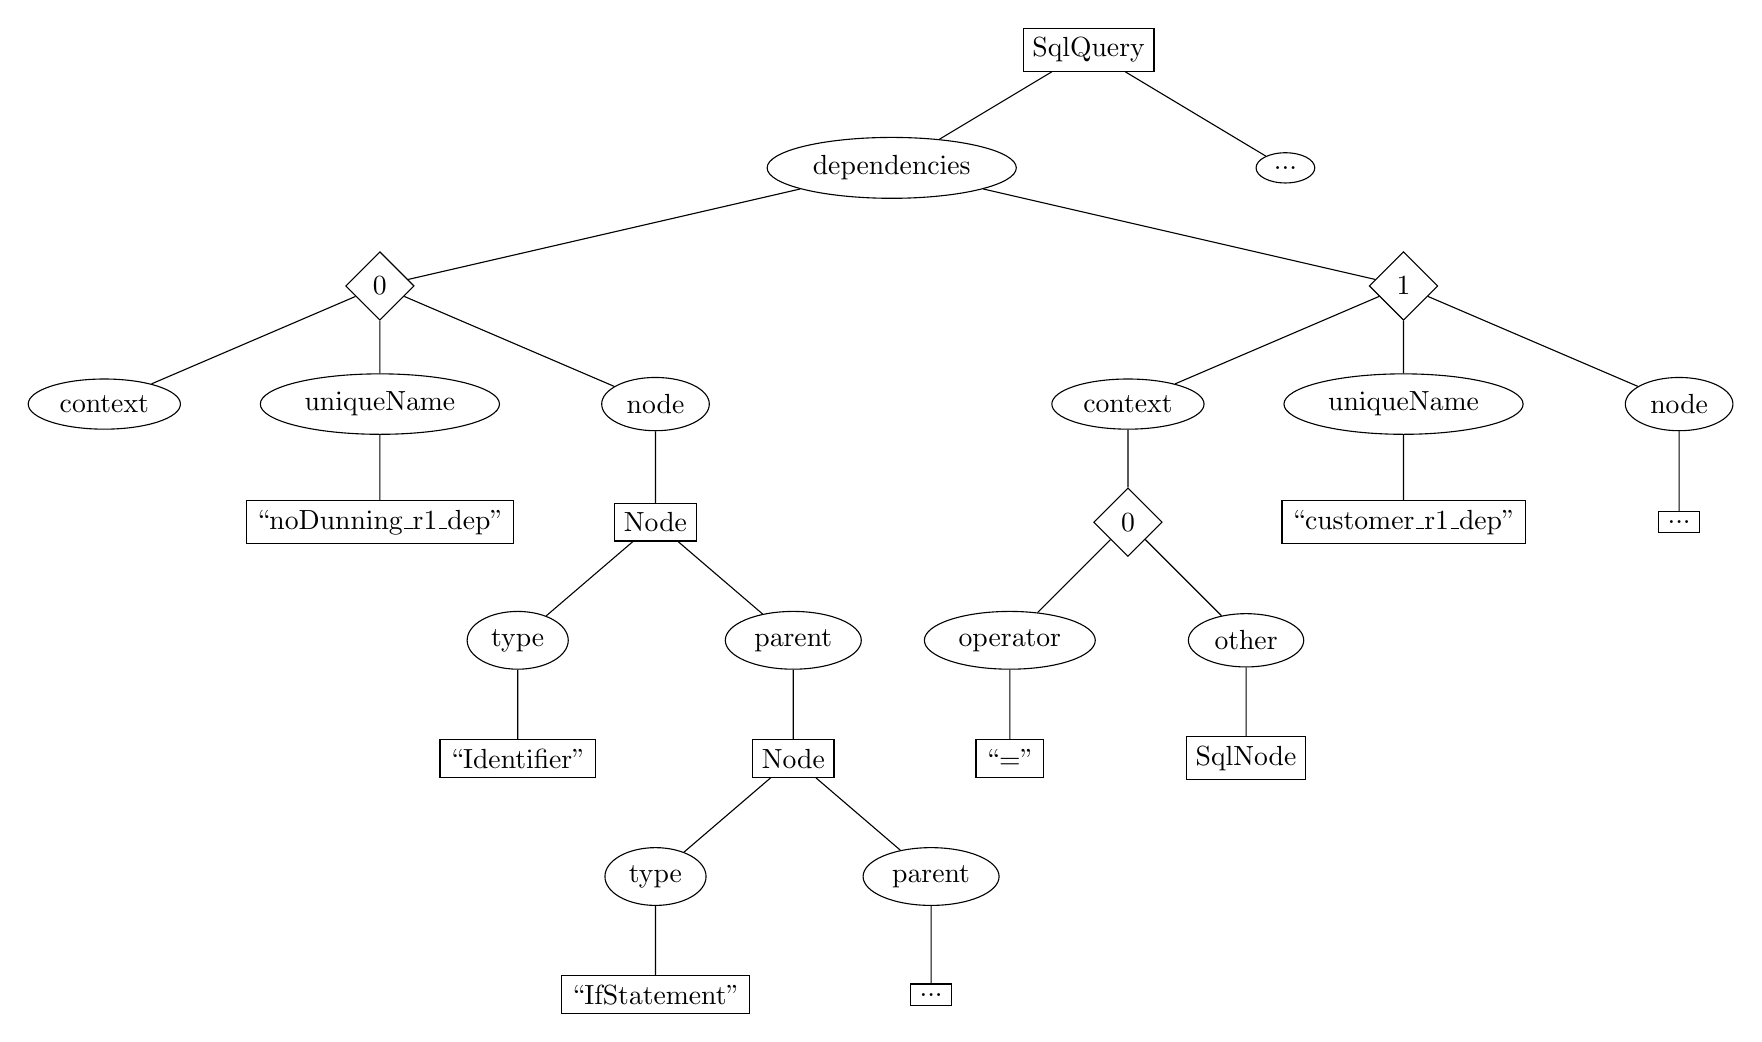
\begin{tikzpicture}
			\usetikzlibrary{shapes}
			\tikzstyle{e} = [draw, shape=ellipse]
			\tikzstyle{r} = [draw, shape=rectangle]
			\tikzstyle{d} = [draw, shape=diamond]
			\node[r] (is-root) {SqlQuery}
				[sibling distance=5cm]
				child {
					node[e] {dependencies}
					[sibling distance=13cm]
					child {
						node[d] {0}
						[sibling distance=3.5cm]
						child { node[e] {context} }
						child {
							node[e] {uniqueName}
							child { node[r] {``noDunning\_r1\_dep''} }
						}
						child {
							node[e] {node}
							child {
								node[r] {Node}
								child {
									node[e] {type}
									child {
										node[r] {``Identifier''}
									}
								}
								child {
									node[e] {parent}
									child {
										node[r] {Node}
										child {
											node[e] {type}
											child {
												node[r] {``IfStatement''}
											}
										}
										child {
											node[e] {parent}
											child {
												node[r] {...}
											}
										}
									}
								}
							}
						}
					}
					child {
						node[d] {1}
						[sibling distance=3.5cm]
						child {
							node[e] {context}
							child {
								node[d] {0}
								[sibling distance=3cm]
								child {
									node[e] {operator}
									child { node[r] {``=''} }
								}
								child {
									node[e] {other}
									child { node[r] {SqlNode} }
								}
							}
						}
						child {
							node[e] {uniqueName}
							child { node[r] {``customer\_r1\_dep''} }
						}
						child {
							node[e] {node}
							child { node[r] {...} }
						}
					}
				}
				child { node[e] {...}
				};
		\end{tikzpicture}
	}

	\vspace{\baselineskip}

	\scalebox{1}{
		\begin{tikzpicture}[framed, node distance=2cm]
			\usetikzlibrary{shapes}
			\tikzstyle{e} = [draw, shape=ellipse]
			\tikzstyle{r} = [draw, shape=rectangle]
			\tikzstyle{d} = [draw, shape=diamond]
			%\node [e] {dependencies};

			\node (title) [font=\bfseries] {Legende:};
			\node [r, right = of title, label=right:{Objekt}] (object) {};
			\node [e, right = of object, label=right:{Attribut}] (attribute) {};
			\node [d, right = of attribute, label=right:{Array-Element}] (array) {};
		\end{tikzpicture}
	}

	\caption{Erweiterung des Baumes aus Abbildung \ref{fig:querytree} für Variablen ohne Datenbankbezug}
	\label{fig:querytreeextended}
\end{figure}

In den erkannten Abhängigkeiten eines SQL-Statements werden zusätzlich ihre Kontextinformationen als Knoten gespeichert.
Diese dienen zur Einordnung innerhalb des vom Quellcodeparser erstellten AST \cite{Horschig2014}.
Durch Betrachtung der Typen der Vorfahren im Baum, in diesem Beispiel des Elternknotens vom Typ ``IfStatement'', können passende Vorschläge erzeugt werden.
Ein Vorschlag für eine Variable umfasst immer 2 Werte: einer, der die assoziierte Bedingung erfüllt und einer, der sie nicht erfüllt.
Tabelle \ref{tab:tableforgeneratedvalues} zeigt für verschiedene Knotentypen und Operatoren die Bestimmung der zwei Wertvorschläge bei Vergleichen mit Literalen.
Für die Variable \texttt{noDunning} sind das \texttt{true} und \texttt{false}.
Ein Vergleich, beispielsweise \texttt{if(amount > 5)} ergibt als Testwerte \texttt{5} (nicht erfüllend) und \texttt{5+1}, also \texttt{6} (erfüllend).
In Abhängigkeit des Vergleichsoperators muss einer der beiden vorgeschlagene Werte angepasst werden um die Negation der Bedingung zu erreichen.

\begin{table}[ht!]
	\centering
	\begin{tabular}{ |l|c|c|c| }
		\hline
		%\multicolumn{2}{|c|}{BSEG-Spalten} \\
		Elternknotentyp 								  & Operator 											& Erfüllender Wert 	& Nichterfüllender Wert\\
		\hline
		\multicolumn{2}{|l|}{IfStatement} 																& \texttt{true} 		& \texttt{false} 	\\
		\hline
		UnaryExpression 								  & \texttt{!} 										& \texttt{true} 		& \texttt{false} 	\\
		\hline
		\multirow{7}{*}{BinaryExpression} & \multirow{3}{*}{\texttt{==}} 	& \texttt{x} 				& \texttt{x+1}		\\ \cline{3-4}
																		  & 															& \texttt{x} 				& \texttt{x+'a'}	\\ \cline{3-4}
																		  & 															& \texttt{x} 				& \texttt{!x}			\\ \cline{2-4}
																		  & \texttt{<} 										& \texttt{x-1} 			& \texttt{x}			\\ \cline{2-4}
																		  & \texttt{<=} 									& \texttt{x} 				& \texttt{x+1}		\\ \cline{2-4}
																		  & \texttt{>} 										& \texttt{x+1} 			& \texttt{x}			\\ \cline{2-4}
																		  & \texttt{>=} 									& \texttt{x} 				& \texttt{x-1}		\\
		\hline
	\end{tabular}
	\caption{Testwertermittlung für Vergleiche einer Variable mit einem Literal \texttt{x}}
	\label{tab:tableforgeneratedvalues}
\end{table}

Der Ansatz ist ähnlich dem Verfahren in Testing-Frameworks, um eine erhöhte Verzweigungsüberdeckung zu erreichen und unterstützt derzeit die drei primitiven Datentypen von JavaScript (Wahrheitswerte, Zahlen, Zeichenketten).

\subsection{Integration in die Web-IDE}
\begin{figure}[ht]
	\centering
  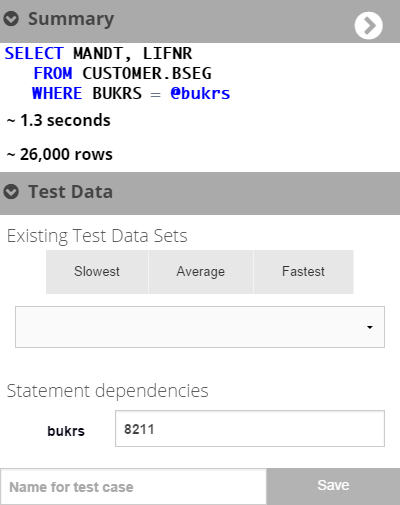
\includegraphics[width=0.4\textwidth]{figures/integration.png}
	\caption{Integration des Werkzeugs in die Sidebar der Web-IDE}
	\label{fig:ideintegration}
\end{figure}

Die in Kapitel \ref{chap:datacharacteristics} und \ref{chap:adaptive} erzeugten Vorschläge werden in der zur Web-IDE gehörenden Datenbank gespeichert und in einer Sidebar im Frontend eingebunden (vgl. Abbildung \ref{fig:ideintegration}).
Durch das Auswählen einer Quellcodezeile mit SQL-Inhalt werden die Informationen zu dem dazugehörigen SQL-Statement aggregiert und aufbereitet (vgl. Kapitel \ref{chap:entwicklungsumgebung}) und schließlich in der Sidebar angezeigt.

Aus der in Kapitel \ref{chap:adaptive} ermittelten Menge an Testdatensets werden zum einen die drei Sets mit der höchsten, geringsten und durchschnittlichen Laufzeit angeboten, zum anderen aber auch ein Menü mit allen gespeicherten Sets zur Auswahl gestellt.
Die Wahl einer dieser Optionen füllt die Eingabefelder für die Testdaten automatisch mit den gespeicherten Werten und löst eine Analyse aus.
Möchte der Entwickler weitere Testdatensets hinzufügen, so kann er diese benennen und direkt abspeichern.
Die Verwaltung solchermaßen gespeicherten Daten wird im folgenden Kapitel behandelt.
